


\chapter{Экспериментальная часть}\label{exp}
%\addcontentsline{toc}{chapter}{4 Экспериментальная часть}

Оценка качества работы алгоритмов. Экспериментальное сравнение работы различных алгоритмов нахождения среднего арифметического матрицы
(зависимость времени выполнения от размерности матриц).

\section{Технические характеристики}\label{texcharacters}

Технические характеристики устройства, на котором выполнялось тестирование:

\begin{enumerate}
    \item процессор: Intel® Core™ i3-7100U CPU @ 2.40GHz × 4; 
    \item память: 11,6 GiB;
    \item операционная система: Ubuntu 20.04.1 LTS.
\end{enumerate}

\section{Примеры работы}\label{examples}

На рисунке \ref{ris:w1} показан пример работы.

\begin{figure}[H]
    \center{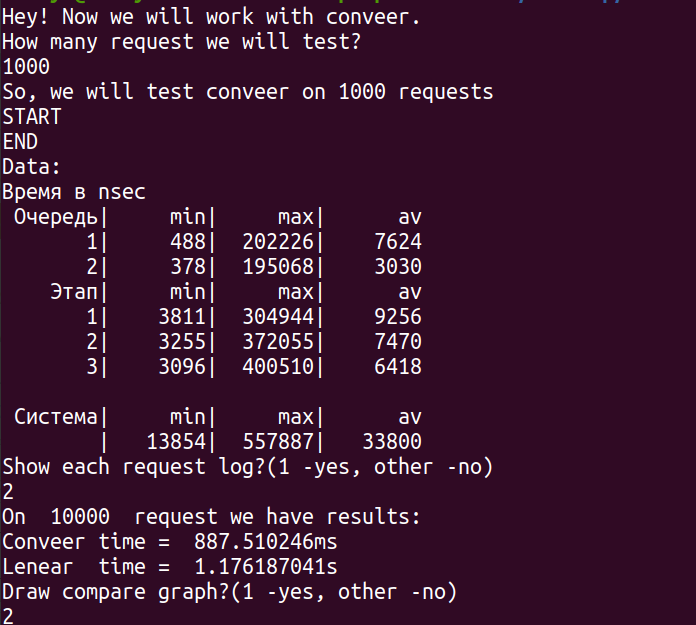
\includegraphics[scale=0.3]{w1}}
    \caption{Пример работы 1}
    \label{ris:w1}
\end{figure}
  
%\begin{figure}[H]
%    \center{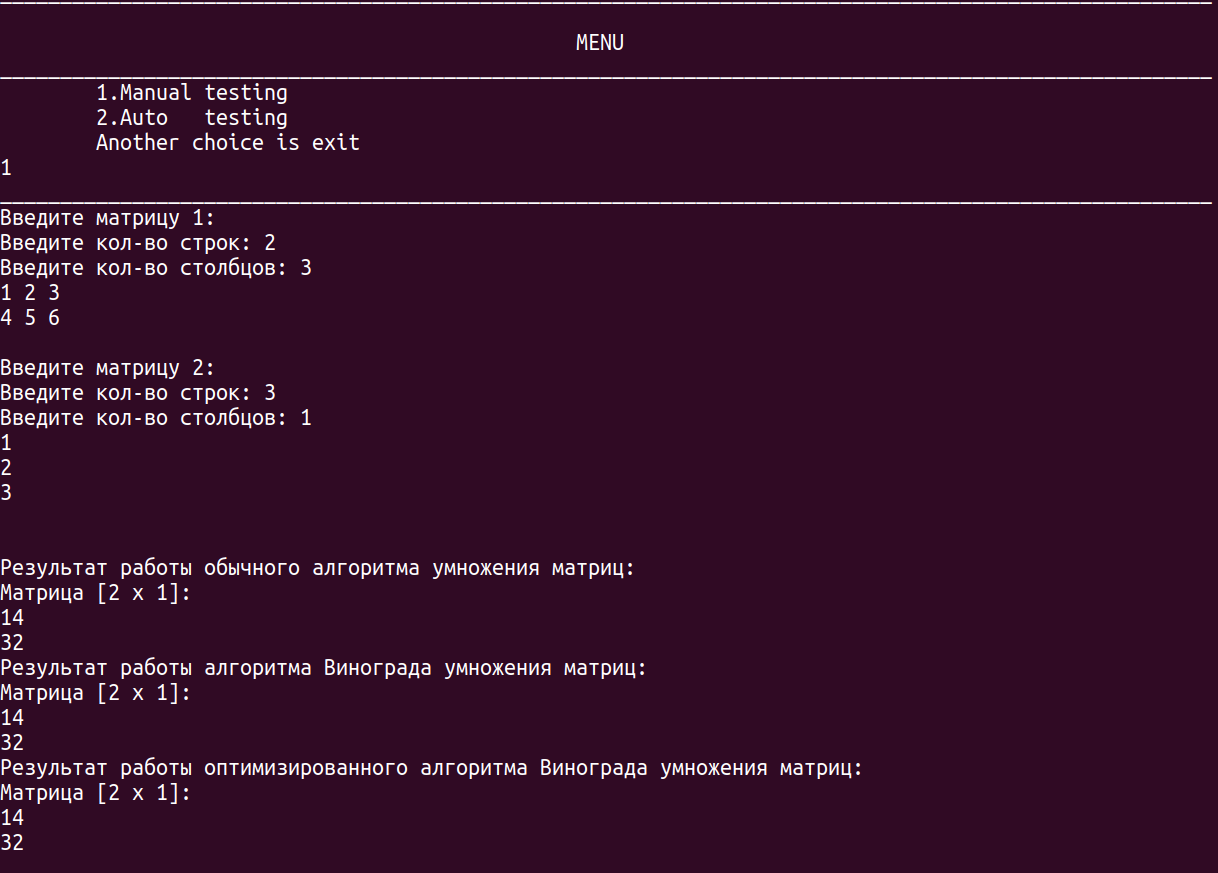
\includegraphics[scale=0.35]{w3}}
%    \caption{Ручное тестирование: тест 3}
%    \label{ris:w4}
%\end{figure}
  
%\begin{figure}[H]
%    \center{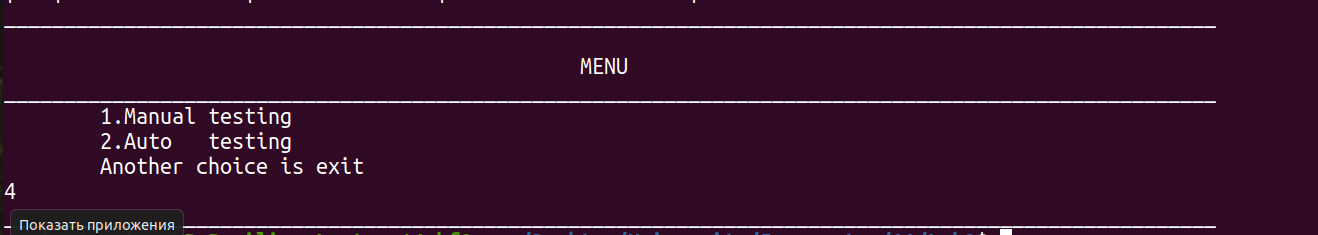
\includegraphics[scale=0.5]{w5}}
%    \caption{Пример работы 3}
%    \label{ris:w3}
%\end{figure}

\newpage

\section{Замеры времени}\label{experimentgraph}

Таблица \ref{tab:resulttime} содержит лог первых 16 заявок.

\begin{table}[ht]
    \caption{Лог заявок (нсек)}
    \centering
    %\scriptsize
\begin{tabular}{ l | l | l | l | l | l | l | l | l }

 id &   go conv &1 step st & 2 step en &1 step st & 2 step en &1 step st & 2 step en \\ \hline
 0 &         0 &    26079 &    664732 &   742436 &    758880 &   772739 &    788061 \\ 
 1 &    121906 &   754064 &    769764 &   874328 &    885545 &   910297 &    921014 \\
 2 &    771362 &   909081 &    919927 &  1000013 &   1012542 &  1138180 &   1147318 \\
 3 &    920734 &  1054765 &   1064300 &  1224065 &   1245139 &  1250378 &   1254853 \\
 4 &   1064843 &  1365380 &   1373496 &  1383268 &   1392493 &  1393559 &   1397981 \\
 5 &   1382654 &  1450067 &   1464613 &  1474740 &   1485290 &  1487019 &   1496701 \\
 6 &   1498192 &  1499075 &   1506823 &  1540792 &   1548461 &  1556604 &   1564338 \\
 7 &   1498602 &  1617884 &   1627640 &  1630647 &   1642891 &  1643533 &   1650580 \\
 8 &   1651564 &  1706643 &   1717353 &  1722394 &   1730959 &  1731787 &   1736708 \\
 9 &   1737951 &  1796989 &   1805167 &  1809310 &   1813951 &  1814601 &   1819223 \\
10 &   1820352 &  1883808 &   1894320 &  1903558 &   1922516 &  1923622 &   1930865 \\
11 &   1902944 &  1968995 &   1974614 &  1978125 &   1990048 &  1990820 &   1995240 \\
12 &   1978034 &  2051845 &   2061071 &  2065122 &   2069918 &  2070621 &   2074851 \\
13 &   2076065 &  2137928 &   2153802 &  2163676 &   2170724 &  2171611 &   2178528 \\
14 &   2162848 &  2228934 &   2240335 &  2244886 &   2249660 &  2250362 &   2254679 \\
15 &   2255685 &  2438950 &   2448361 &  2456493 &   2465216 &  2466067 &   2471479 \\

\end{tabular}
\label{tab:resulttime}
\end{table}

Таблица \ref{tab:resulttime2} содержит минимальное, максимальное и среднее время пребывания заявки в очередях, в этапах и в конвейере.

\begin{table}[ht]
    \caption{Статистика времени пребывания заявок (нсек)}
    \centering
    %\scriptsize
\begin{tabular}{ l | l | l | l  }
  Очередь&     min&     max&      av \\\hline
  1&     488&  202226&    7624 \\
  2&     378&  195068&    3030 \\ \hline
Этап&     min&     max&      av \\ \hline
  1&    3811&  304944&    9256 \\
  2&    3255&  372055&    7470 \\
  3&    3096&  400510&    6418 \\ \hline

Система&     min&     max&      av \\ \hline
   &   13854&  557887&   33800 \\

\end{tabular}
\label{tab:resulttime2}
\end{table}

Таблица \ref{tab:resulttime3} содержит время работы конвейрной обработки и стандартного алгоритма.

\begin{table}[ht]
    \caption{Время работы конвейрной обработки и стандартного алгоритма (нсек)}
    \centering
    %\scriptsize
\begin{tabular}{| l | l | }
    \hline
    Алгоритм & Время \\ \hline
    Conveer &  911.49707ms \\
    Lenear  &  1.184577591s \\ \hline
\end{tabular}
\label{tab:resulttime3}
\end{table}

На рисунках \ref{ris:graph1} и \ref{ris:graph2} показаны графические результаты сравнения исследуемых алгоритмов по времени. 

\begin{figure}[H]
    \center{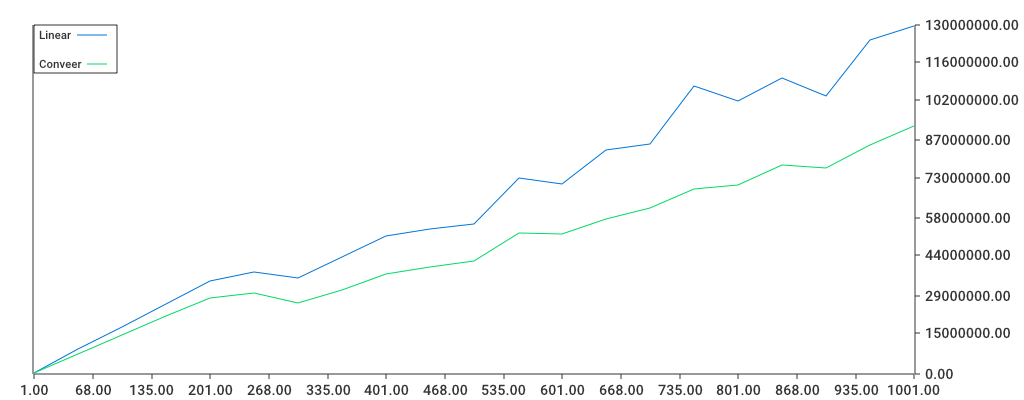
\includegraphics[scale=0.45]{graph}}
    \caption{Сравнение конвейерной обработки и последовательного алгоритма}
    \label{ris:graph1}
\end{figure}

\begin{figure}[H]
    \center{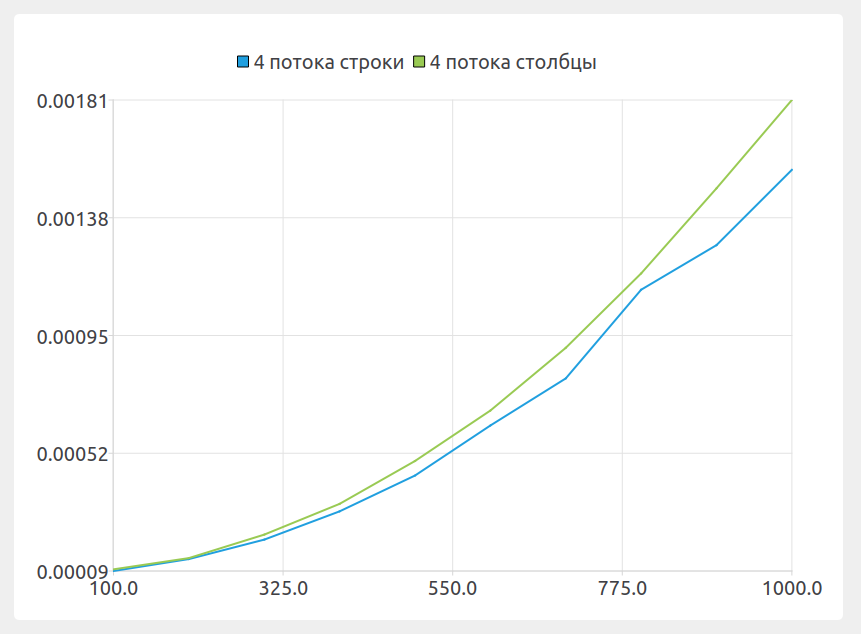
\includegraphics[scale=0.4]{graph2}}
    \caption{Время пребывания заявок во второй и третьей очередях}
    \label{ris:graph2}
\end{figure}

\section{Сравнительный анализ}\label{expE}

По результатам экспериментов можно заключить следующее:

\begin{itemize}
    \item конвейерная обработка быстрее обычной;
    \item из времени пребывания заявок в 2 и 3 очередях следует, что 3 этап быстрее 2;
    \item первый этап самый медленный из всех;
    \item третий этап самый быстрый.
\end{itemize}


\section{Вывод экспериментальной части}\label{experimentresult}

В данном разделе были рассмотрены результаты работы программы.
Из анализа стало ясно, что первый этап - шифрование с помощью шифра
Цезаря замедляет работу всей системы. Самым быстрым является шифрование xor.


\addcontentsline{toc}{chapter}{{Заключение}}
\chapter*{Заключение}\label{exit}

В ходе лабораторной работы достигнута поставленная цель: разработ-
ка и исследование конвейерных вычислений и использование их на практике.
Также решены все поставленные задачи.
Получены практические навыки реализации конвейера. 
Проведёно исследование конвейерных вычислений и использование их на практике. 
Экспериментально подтверждены различия в эффективности алгоритмов с указанием лучших и худших случаев.
Цель работы достигнута, решены поставленные задачи. 
